\documentclass[12pt, a4paper]{article}

% Acentuação
\RequirePackage[T1]{fontenc}
\RequirePackage[utf8]{inputenc}

% Configurando as margens
\usepackage[top = 2cm, bottom = 2cm, left = 3cm, right = 3cm]{geometry}
% Indentação do parágrafo
\setlength{\parindent}{2cm}
% Espaçamento entre parágrafo e texto
\setlength{\parskip}{1em}
% Espaçamento entre linhas
\renewcommand{\baselinestretch}{1.5}
% Identar o primeiro parágrafo das seções
\usepackage{indentfirst}
% Para usar símbolos como >=
\usepackage{amssymb}
% Para colocar texto entre $$ com \text{oi}
\usepackage{amsmath}
% Para usar listas com estilos específicos
\usepackage{enumerate}
% Para utilizar imagens
\usepackage{graphicx}

\renewcommand{\figurename}{Figura}

\begin{document}

	\input{Título.tex}

	\section{Introdução à pilares}
	Em estruturas de edifícios, os pilares são elementos verticais que tem a função primária de transmitir as \textbf{ações verticais} gravitacionais e de serviço e as \textbf{orizontais (vento)} às fundações, além de conferirem \textbf{estabilidade global} ao edifício. Os pilares usuais dos edifícios apresentam um comportamento de flexo-compressão, sendo as forças normais preponderantes.
Em edifícios de concreto armado, as seções dos pilares são geralmente \textbf{retangulares}.

% inserir imagem

Pilares de seção \textbf{quadrada} ou \textbf{circular} também podem ser considerados em projetos estruturais de edifícios.
Em virtude do tipo de material (concreto) e da solicitação preponderantemente de força de compressão, os pilares apresentam \textbf{rupturas frágeis}. A \textbf{ruína} de uma seção transversal de \textbf{um único pilar} pode ocasionar o \textbf{colapso} progressivo dos demais pavimentos.

As \textbf{disposições} dos pilares na planta de forma de um edifício são importantes, pois, junto com as vigas, formam \textbf{pórticos} que proporcionam \textbf{rigidez} e \textbf{estabilidade global} ao edifício.

Os pilares são peças estruturais que precisam ser projetadas \textbf{cuidadosamente} em termos de resistência, estabilidade e durabilidade, sempre respeitando as diretrizes e recomendações das \textbf{normas técnicas}.

O dimensionamento dos pilares é feito em função dos esforços externos solicitantes de cálculo, que compreendem as forças normais $(N_d)$ e os momentos fletores $(M_{dx}$ e $M_{dy})$.

	\section{Agressividade do ambiente}
	Está relacionada às \textbf{ações físicas} e \textbf{químicas} que atuam sobre as estruturas de concreto, independentemente das \textbf{ações mecânicas}, das variações térmicas, da retração e outras previstas no dimensionamento das estruturas.

Nos projetos das estruturas, a agressividade ambiental deve ser classificada de acordo com a Tabela 6.1 da ABNT NBR 6118 e pode ser avaliada segundo as condições de exposição da estrutura ou de suas partes. Conhecendo o ambiente em que a estrutura será construída, o projetista estrutural pode considerar uma condição de agressividade maior que a tabela.

% inserir tabela

Conforme a NBR 6118 - item 7.4: A durabilidade das estruturas é \textbf{altamente dependente} das características do concreto e da \textbf{espessura} e \textbf{qualidade} do concreto de cobrimento da armadura.

\textbf{Ensaios comprobatórios} de desempenho da durabilidade da estrutura frente ao tipo e classe de agressividade prevista em projeto devem estabelecer os parâmetros mínimos a serem atendidos. Na falta destes e devido à existência de uma \textbf{forte correspondência} entre a \textbf{relação água/cimento} e a \textbf{resistência do concreto} e sua \textbf{durabilidade}, permite-se que sejam adotados os requisitos mínimos da tabela abaixo:

\begin{table}[H]
\centering
\caption{Tabela 7.1 da NBR 6118.}
\begin{tabular}{|c|c|c|c|c|}
\hline
\multirow{2}{*}{Concreto} & \multicolumn{4}{c|}{Classe de Agressividade Ambiental (CAA)}                      \\ \cline{2-5} 
                          		& I                  & II                 & III                & IV                 \\ \hline
Relação a/c               & $\leqslant$ 0,65   & $\leqslant$ 0,6    & $\leqslant$ 0,55   & $\leqslant$ 0,45   \\ \hline
Classe de concreto        & $\geqslant$ C20 & $\geqslant$ C25 & $\geqslant$ C30 & $\geqslant$ C40 \\ \hline
\end{tabular}
\end{table}

	\section{Solicitações normais}
	Os pilares podem estar submetidos à forças normais e momentos fletores, gerando compressão simples e flexão composta.

\begin{itemize}

	\item \textbf{Compressão simples}: Também chamada de compressão centrada ou compresão uniforme, é caracterizada pela aplicação da força normal $(N_d)$ no centro geométrico da seção transversal do pilar.

		\begin{figure}[H]
			\begin{center}
				\caption{Solicitação normal acontecendo no centro geométrico da seção transversal do pilar.}    	
				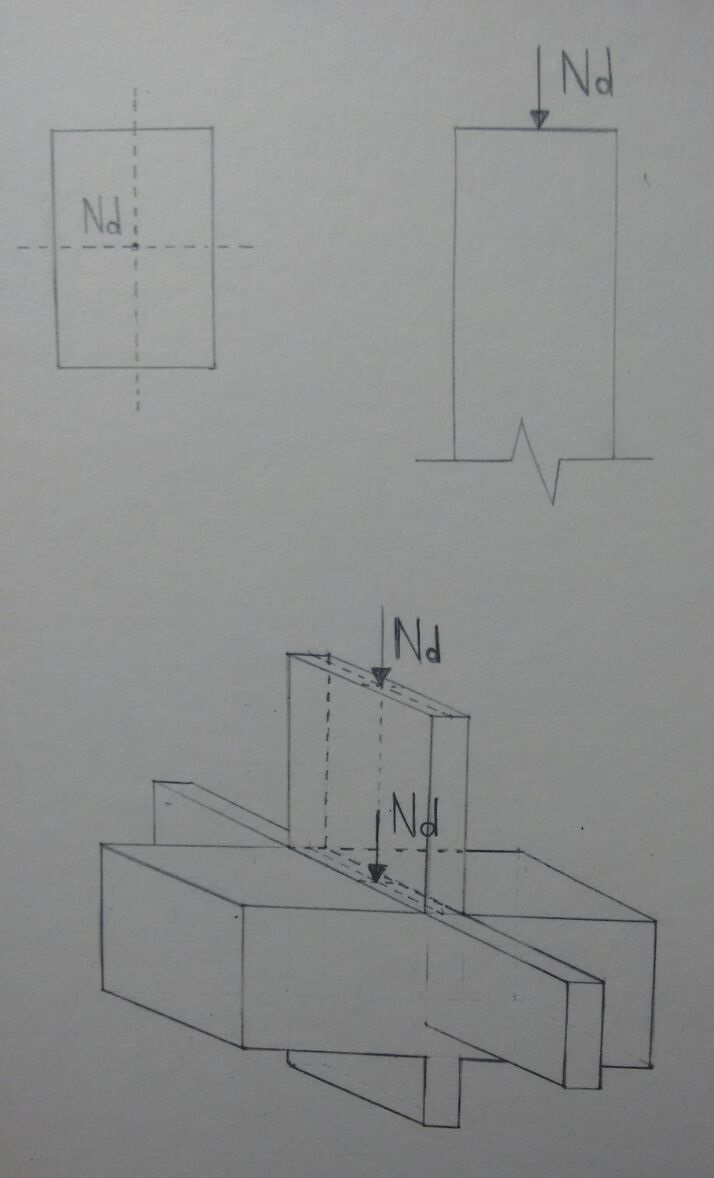
\includegraphics[height=0.5\textwidth]{Solicitacoes-normais/Imagens/Compressao-simples.jpg}
			\end{center}
		\end{figure}

	\item \textbf{Flexão composta}: Ocorre força normal e momento fletor sobre o pilar. Há dois casos:

		\begin{itemize}
     			\item \textit{Flexão composta normal (ou reta)}: Existe a força normal e um momento fletor em uma direção, sendo:
				$$M1_{dx}=e1_x\cdot N_d$$
				
     			\item \textit{Flexão composta oblíqua}: Existe força normal e dois momentos fletores, sendo:
				$$M1_{dx}=e1_x\cdot N_d$$
				$$M1_{dy}=e1_y\cdot N_d$$
  		\end{itemize}

\end{itemize}



	\section{Carga sobre pilares}
	Durante o desenvolvimento e desenho da planta de fôrma é necessário definir as dimensões dos pilares, antes mesmo que se conheçam os esforços solicitantes atuantes. Alguns processos podem ser utilizados para fixação das dimensões dos pilares, entre eles, a \textbf{experiência} do engenheiro. Outro processo simples que auxilia na fixação das dimensões do pilar é a estimativa da carga vertical no pilar pela sua área de influência, ou seja, a carga que estiver na laje dentro da área de influência do pilar "caminhará" até o pilar.

No entanto, é necessário ter um valor que represente a carga total por metro quadrado de laje, levando-se em conta todos os carregamentos \textbf{permanentes} e \textbf{variáveis}. Para edifícios com fins residenciais e de escritórios, pode-se estimar a carga total de \textbf{$8$} a $10$ $kN/m^2$ ou $800$ a $1000$ $kgf/m^2$ para pisos e $600$ a $800$ $kgf/m^2$ para cobertura. Edifícios com outros fins podem ter \textbf{cargas superiores} e edifícios onde a ação do \textbf{vento} é significativa, a carga por metro quadrado deve ser majorada.

Lembrando que essa carga de piso é em \textbf{um andar}. A cada andar para baixo esses valores vão sendo \textbf{agregados}. É importante salientar que a carga estimada serve apenas para o pré-dimensionamento da seção transversal dos pilares. O dimensionamento final deve ser obrigatoriamente feito com os \textbf{esforços reais} calculados em função das cargas das vigas e lajes sobre o pilar, e com a atuação das forças do vento e outras que existirem.

A carga do pilar pode ser obtida atraves da fórmula:
\begin{equation}N_k=[(q+g)\cdot A_{inf}\cdot n]+(A_{inf}\cdot g_{cobertura})\end{equation}

Onde $N_k$ é a carga do pilar em $kgf$, $A_{inf}$ é a área de influência do pilar em $m^2$, $q$ é a carga de utilização do ambiente em $kgf/m^2$, $g$ é a carga do peso próprio em $kgf/m^2$ e $n$ é o número de pavimentos acima da seção analisada.

A carga do pilar também pode ser obtida quando se tem os cálculos de força cortante das vigas, as quais já receberam as cargas das lajes.

	\section{Efeitos de 1ª e 2ª ordem}
	As estruturas de concreto armado devem ser projetadas, construídas e utilizadas de modo que, sob condições ambientais previstas e respeitadas as condições de manutenção preventiva especificadas no projeto, conservem sua \textbf{segurança}, \textbf{estabilidade} e \textbf{aparência aceitável}, sem exigir medidas extras de manutenção e reparo.

Há duas formas de se analisar estruturalmente uma edificação:

\begin{itemize}
	\item Análise linear;
	\item Análise não-linear.
\end{itemize}

Se fosse feita uma análise puramente linear, o \textbf{deslocamento} resultante seria \textbf{proporcional} ao acréscimo de carga.

A resposta da estrutura em termos de deslocamentos teria um comportamento \textbf{linear} à medida que o carregamento fosse aplicado.

Por outro lado, se fosse efetuada uma análise não-linear, o deslocamento resultante \textbf{não seria proporcional} ao acréscimo de carga. E mais, provavelmente seria \textbf{maior} que o encontrado na análise linear.

Pode-se dizer que uma \textbf{análise não-linear} é um cálculo no qual a resposta da estrutura, seja em deslocamentos, esforços ou tensões, possui um comportamento \textbf{desproporcional} à medida que um carregamento é aplicado.

Os fatores que tornam as análises não-lineares importantes no projeto estrutural de edifícios de concreto armado são:

\begin{itemize}
	\item O concreto armado é um material que possui um comportamento \textbf{essencialmente} não-linear;
	\item Pelas análises não-lineares, é possível simular o comportamento de um edifício de concreto armado de forma muito mais \textbf{realista};
	\item Os elementos estruturais estão cada vez mais \textbf{esbeltos}, de tal forma que as \textbf{não-linearidades}, em muitos casos, passam a ser \textbf{preponderantes}.
\end{itemize}

Dois fatores que geram o comportamento não-linear de uma estrutura à medida que o carregamento é aplicado:

\begin{itemize}
	\item \textbf{Não-linearidade física}: Alteração das \textbf{propriedades} dos materiais que compõem a estrutura;
	\item \textbf{Não-linearidade geométrica}: Alteração da geometria da estrutura.
\end{itemize}

	\section{Não-linearidade física}
	O material é linear quando obedece à Lei de Hooke, ou seja, quando a tensão é proporcional à deformação $(\sigma=E\cdot \epsilon)$. Considerando-se uma estrutura de concreto armado, a não-linearidade física resulta da resposta não-linear do \textbf{aço} e do \textbf{concreto}.

Além do comportamento não-linear dos materiais, existe um outro fator que é preponderante na análise de edifícios: a \textbf{fissuração}. Por causa da baixa resistência do concreto à tração, é comum o surgimento de fissuras à medida que o carregamento é aplicado à estrutura.

A NBR 6118 - item 15.3: "Princípios básicos de cálculo" é bem clara: a não-linearidade física, presente nas estruturas de concreto armado, deve ser obrigatoriamente considerada.

	\section{Não-linearidade geométrica}
	Ocorre em razão de mudanças na \textbf{geometria} dos elementos estruturais à medida que um carregamento é aplicado à estrutura.

Para que a influência da não-linearidade geométrica na análise de uma estrutura seja compreendida, é necessário entender o que são os \textbf{efeitos de segunda ordem}.

A condição de equilíbrio sempre foi considerada na configuração geométrica \textbf{inicial} da estrutura, isto é, na sua posição \textbf{não-deformada}. Esta análise se chama \textbf{Análise de primeira ordem} e os seus efeitos (deslocamentos e esforços resultantes) são chamados de \textbf{Efeitos de primeira ordem}.

Ao admitir o equilíbrio na configuração \textbf{indeformada}, passa-se a se fazer uma aproximação. Porém, na realidade, o equilíbrio de uma estrutura se dá \textbf{sempre} numa configuração \textbf{deformada}.

A análise do equilíbrio de uma estrutura na sua posição deformada é denominada de \textbf{Análise de segunda ordem} e os seus efeitos são chamados de \textbf{Efeitos de segunda ordem}.

A análise de 1ª ordem é uma aproximação que pode ser perfeitamente utilizada pelo fato de os efeitos de 2ª ordem, em muitos casos, \textbf{serem desprezíveis} (quando não apresentam acréscimo superior a 10\% nas solicitações em relação aos efeitos de 1ª ordem).

No entanto, existem certas situações em que os efeitos de 2ª ordem necessitam, obrigatoriamente, serem considerados, tais como:

\begin{itemize}
	\item Análise da estabilidade global;
	\item Cálculo dos esforços para dimensionamento dos pilares.
\end{itemize}

\begin{figure}[H]
	\begin{center}
	\caption{Efeitos de 1ª ordem à esquerda e Efeitos de 2ª ordem à direita.}
    	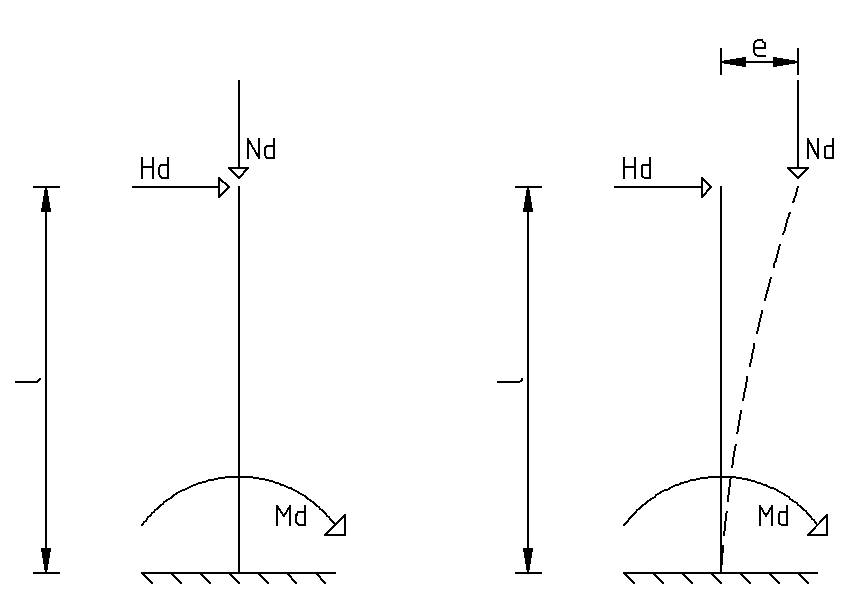
\includegraphics[width=0.5\textwidth]{Nao-linearidade-geometrica/Imagens/Efeitos-de-1a-e-2a-ordem.png}
	\end{center}
\end{figure}

\end{document}